\chapter{Pipeline}\label{ch:pipeline}
%This chapter presents a detailed examination of a multi-stage NLP pipeline designed to enhance information retrieval and question answering capabilities.
%The pipeline integrates various cutting-edge technologies and methodologies, creating a synergistic system that pushes the boundaries of what is possible in automated information processing and response generation.
%However, the challenges of accurately interpreting user queries, retrieving relevant information from vast datasets, and generating coherent and contextually appropriate responses remain significant.
%This pipeline addresses these challenges through a carefully orchestrated series of processes, each designed to refine and enhance the quality of information flow from input to output.
%
%At its core, the pipeline leverages a knowledge graph dataset, serving as the foundational repository of interconnected information.
%This graph structure allows for the representation of complex relationships between entities, facilitating more nuanced understanding and retrieval of information.
%The pipeline then employs a series of sophisticated mechanisms, including query generation, cross-encoding for relevance assessment, and multi-tiered information retrieval strategies, to navigate this knowledge landscape effectively.
%
%One of the key innovations in this pipeline is its approach to context processing and information synthesis.
%By breaking down retrieved information into manageable chunks and employing advanced embedding techniques, the system can perform more granular and accurate analyses of textual data.
%This granularity, combined with the implementation of multiple LLMs working in concert, allows for a more robust and nuanced interpretation of complex queries and generation of comprehensive responses.
%
%The integration of external information sources, notably through the incorporation of Google Search capabilities, further enhances the pipeline's ability to access and process up-to-date and diverse information.
%This hybrid approach, combining structured knowledge graphs with dynamic web-based information retrieval, positions the pipeline at the forefront of adaptive and responsive AI systems.
%
%Critical to the pipeline's effectiveness is its sophisticated decision-making architecture.
%Employing strategies such as majority voting among multiple models and the implementation of a final judge for conflict resolution, the system strives to achieve a balance between diverse perspectives and the need for coherent, unified outputs.
%This approach not only enhances the accuracy and reliability of the generated responses but also provides a framework for managing the inherent uncertainties and potential biases in AI-driven decision-making processes.
%
%As we delve deeper into each component of this pipeline, it is crucial to maintain a critical perspective on both its capabilities and limitations.
%While the system represents a significant advancement in NLP and information retrieval technologies, it also raises important questions about the ethical implications of AI-driven information processing, the potential for bias in knowledge representation and model training, and the broader societal impacts of increasingly sophisticated question-answering systems.

This chapter outlines a multi-stage NLP pipeline developed specifically for fact verification.
The pipeline integrates advanced technologies and methodologies to address core challenges in verifying information accuracy, interpreting user queries, retrieving relevant data from large datasets, and generating factually consistent responses.

The pipeline's foundation is a knowledge graph dataset, which captures complex relationships between entities to support in-depth retrieval and verification.
The pipeline applies query generation, cross-encoding for relevance, and multi-layered retrieval strategies to effectively analyze and cross-check information against this structured data.

To access diverse and up-to-date sources, the pipeline incorporates Google Search, blending structured knowledge with real-time information retrieval to enhance verification accuracy.

A key feature of the pipeline is its approach to context processing and information synthesis.
By dividing retrieved data into manageable sections and utilizing embedding techniques, the pipeline performs precise analyses, enabling a robust assessment of facts with the support of multiple LLMs, and ensuring thorough verification.

The decision-making framework in the pipeline leverages majority voting across models and employs a final judge to resolve inconsistencies, creating a balanced and coherent output.
This approach helps reduce errors and manage potential biases, strengthening the reliability of verified information.

As each pipeline component is further explored, critical insights into its strengths and limitations are addressed.
This includes ethical considerations in AI-driven fact verification, potential biases in knowledge representation, and the broader impacts of advanced verification systems.
\begin{figure}[ht!]
    \centering
    \begin{minipage}[b]{\textwidth}
        \centering
        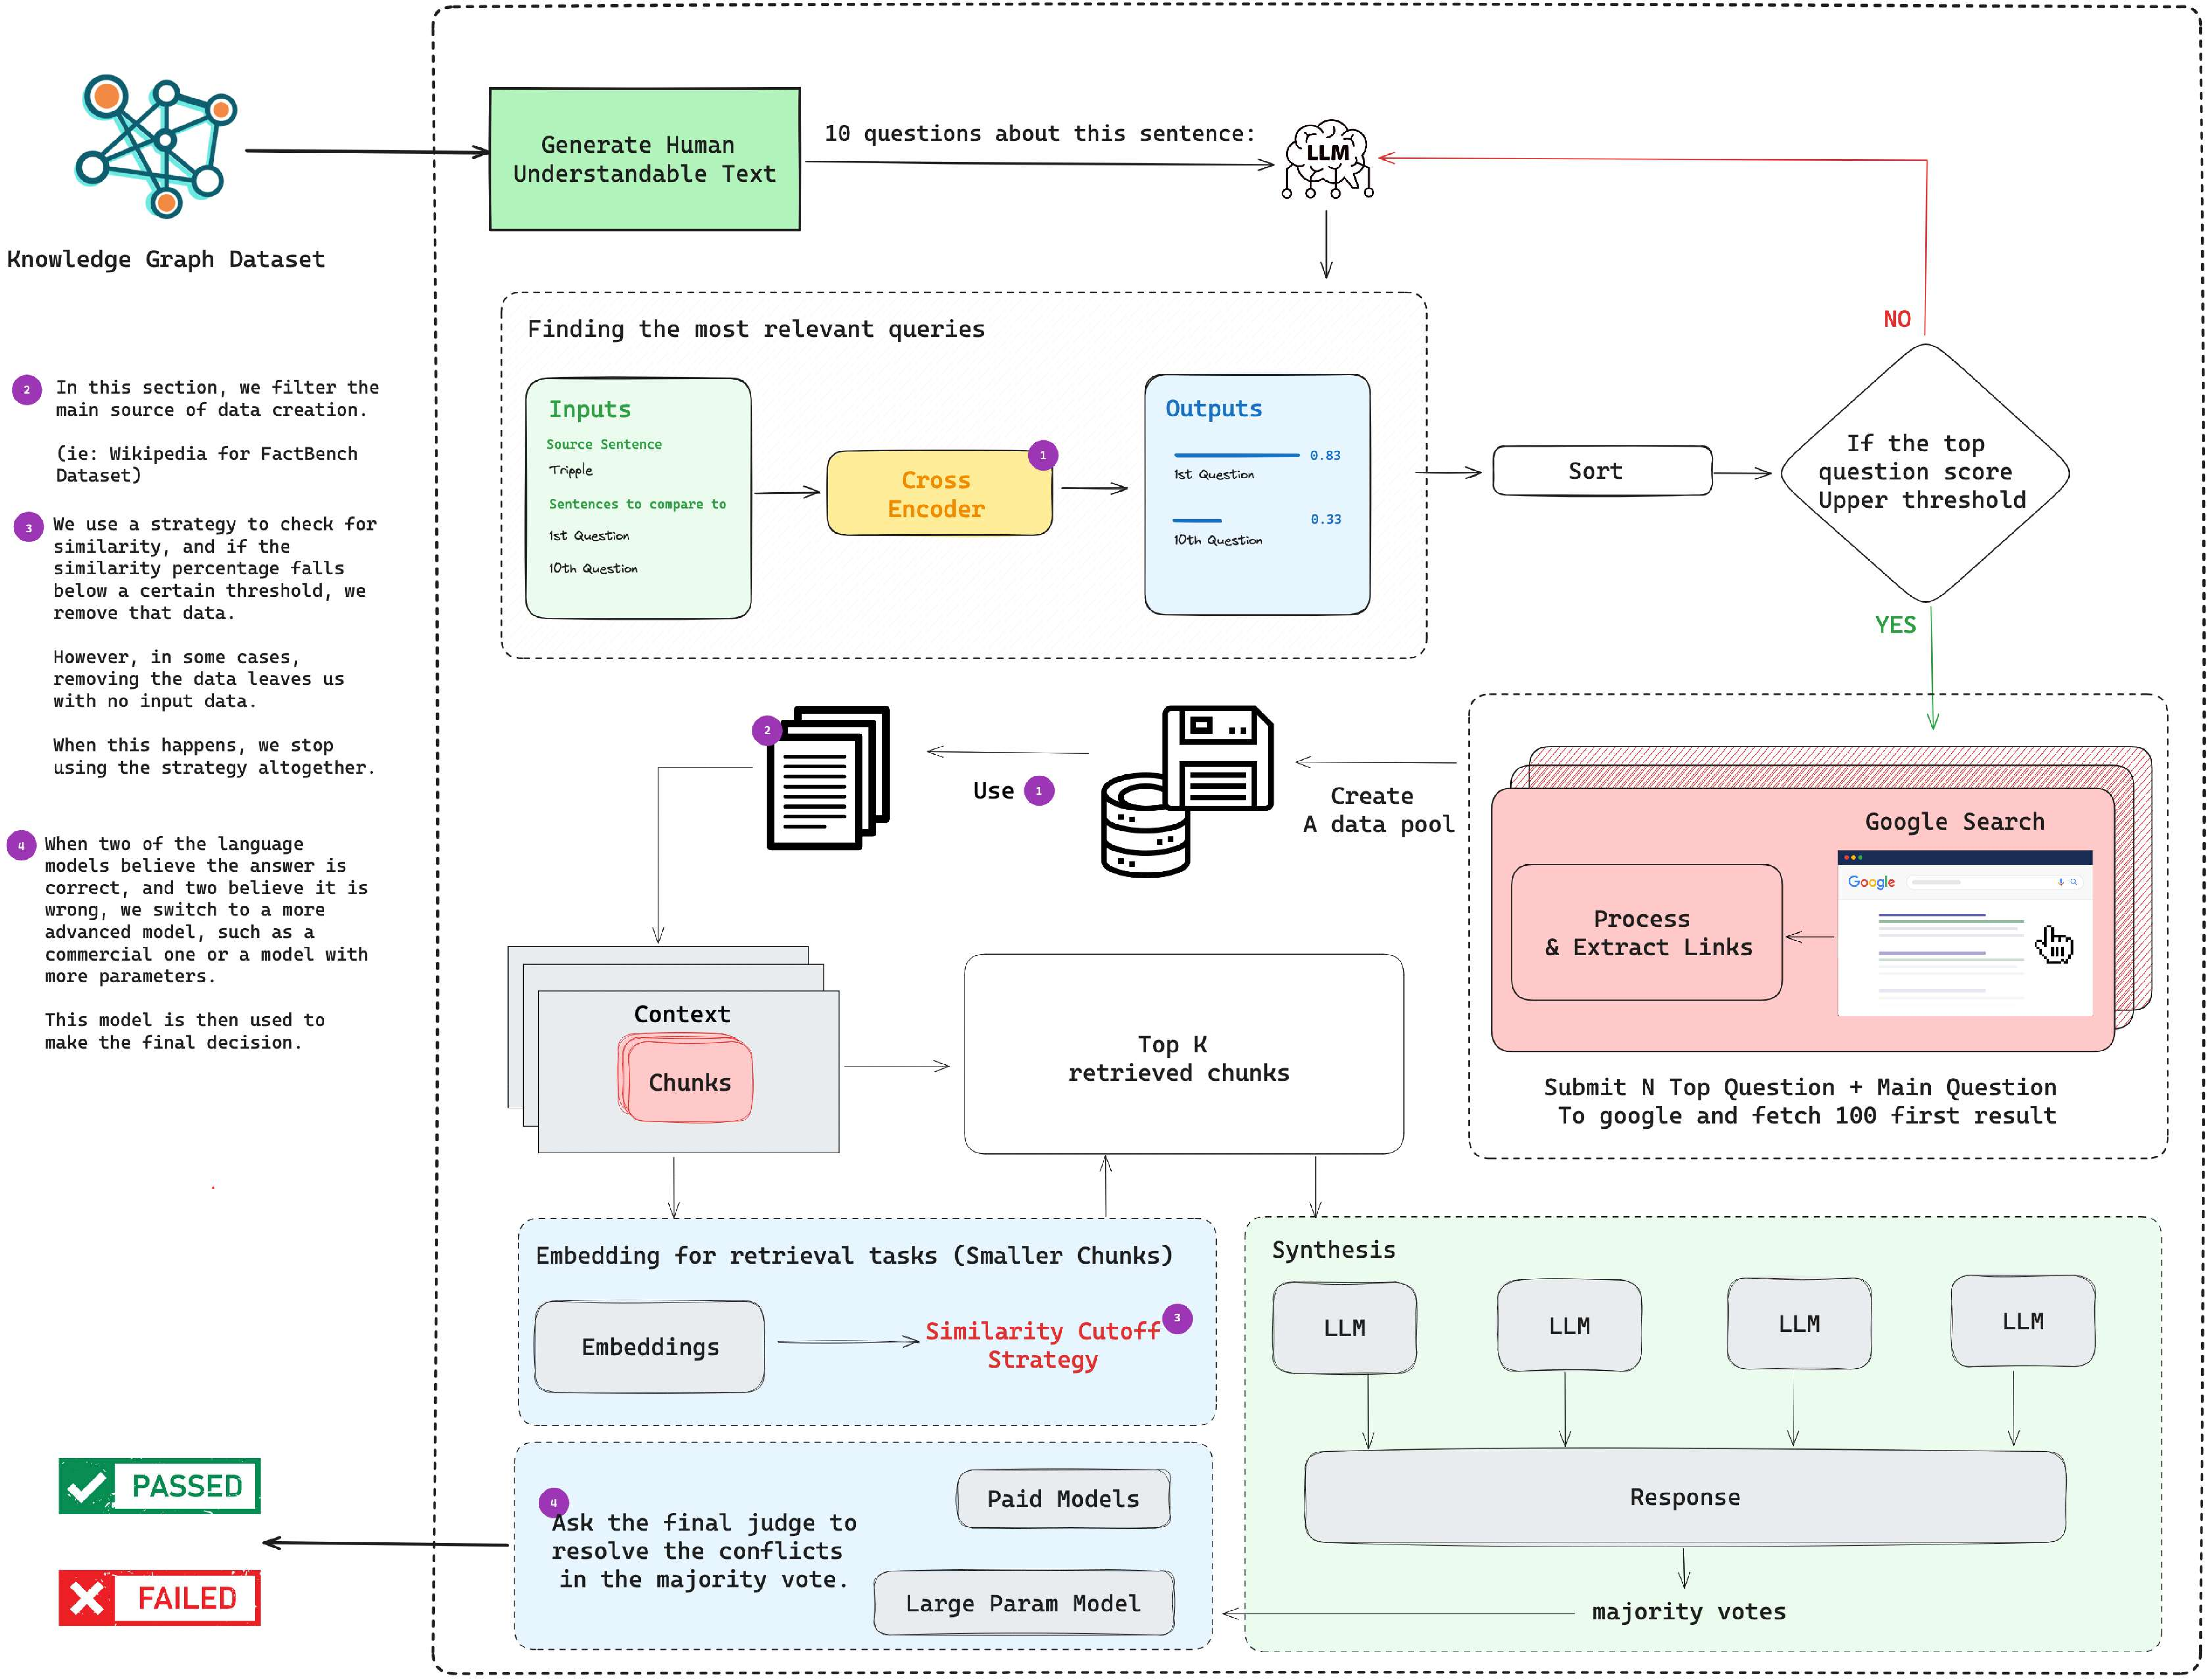
\includegraphics[width=\textwidth]{res/pipeline}
        \caption{RAG-based fact verification pipeline}
        \label{fig:pipeline}
    \end{minipage}
\end{figure}

This chapter aims to provide a comprehensive analysis of each stage of the pipeline as showed on Figure~\ref{fig:pipeline}, examining not only the technical aspects of its implementation but also the theoretical underpinnings and practical implications of its design choices.
By understanding the intricacies of this system, we can gain valuable insights into the current state of NLP technologies and the potential future directions for research and development in this rapidly advancing field.
As we proceed, we will explore each component in detail, starting with the foundational knowledge graph dataset and progressing through the various stages of query processing, information retrieval, context analysis, and response generation.
This exploration will shed light on the complex interplay between different AI technologies and methodologies, offering a holistic view of how modern NLP systems can be architected to tackle some of the most challenging problems in information processing and human-computer interaction.

\section{Knowledge Graph Dataset}\label{sec:knowledge-graph-dataset}
The foundation of our multi-stage RAG pipeline is the Knowledge Graph Dataset, which acts as the primary source of factual information for the ensuing processing stages.
This section clarifies the attributes and aims of the knowledge graph and its use in our pipeline.

\subsection{Definition and Purpose}\label{subsec:definition-and-purpose}
In the form of a graph, a knowledge graph is an ordered way to show information that models real-world things and how they relate to each other.
The Knowledge Graph Dataset is a huge collection of facts, ideas, and connections that are all linked together in our process.
Its main job is to give a lot of background information so that complicated queries can be understood and processed.

The implementation of a knowledge graph fulfills multiple essential functions:
\begin{itemize}
    \item \textbf{Semantic Representation:} Unlike traditional relational databases, knowledge graphs capture semantic relationships between entities, allowing for more nuanced and context-aware information retrieval.
    \item \textbf{Inferential Capabilities:} The interconnected nature of the graph enables the system to make inferences and connections that may not be explicitly stated, enhancing the depth and breadth of responses.
    \item \textbf{Scalability:} Knowledge graphs can efficiently handle large volumes of heterogeneous data, making them ideal for systems that need to process diverse types of information.
    \item \textbf{Flexibility:} The graph structure allows for easy updates and expansions, ensuring that the knowledge base can evolve with new information and changing requirements.
\end{itemize}

\subsection{Structure and Components}\label{subsec:structure-and-components}
The Knowledge Graph Dataset in our pipeline is composed of several key components:
\begin{itemize}
    \item \textbf{Nodes:} Representing entities or concepts, nodes are the fundamental units of information in the graph. Each node typically corresponds to a distinct piece of knowledge, such as a person, place, event, or abstract concept.
    \item \textbf{Edges:} These are the connections between nodes, representing relationships or interactions. Edges are often directional and labeled to indicate the nature of the relationship (\ex, "is\_a", "part\_of", "created\_by").
    \item \textbf{Properties:} Nodes and edges can have associated properties or attributes that provide additional details or metadata about the entity or relationship.
\end{itemize}

\subsection{Role in the Overall Pipeline}\label{subsec:role-in-the-overall-pipeline}
As illustrated in the pipeline diagram, the Knowledge Graph Dataset is the thing that we want to verify the correctness of it.
The pipeline uses the knowledge graph to generate queries, retrieve relevant information, and synthesize responses to find the correctness of the knowledge graph.

\section{Query Generation and Processing}\label{sec:query-generation-and-processing}
The Query Generation and Processing step, following to the basic Knowledge Graph Dataset, is a pivotal point in our pipeline, wherein user inputs are converted into structured queries suitable for efficient processing by later components.
This section clarifies the techniques and methodologies utilized in this critical phase for subsequent actions in the information retrieval process.

\subsection{Human-Understandable Text Generation}\label{subsec:human-understandable-text-generation}
In the first step of the pipeline, we use a LLM (\ie LLama3~\cite{dubey2024llama3herdmodels}, Gemma2~\cite{gemmateam2024gemma2improvingopen}) to easily generate human-readable text by submitting prompts.
This approach bridges the gap between representing raw data and conveying it in natural language, making the information more accessible and understandable.
For additional information, consult the prompt template in Appendix~\ref{sec:prompt-templates:human-understandable} to observe the sentence generation process.

Key aspects of this process include:
\begin{itemize}
    \item \textbf{Contextual Awareness:} Integrating relevant context from the Knowledge Graph to guarantee that the output content is relevant and useful.
    \item \textbf{Adaptability:} Customizing the generated text to accommodate various complexity levels, catering to diverse user needs and query types.
    \item \textbf{Semantic Enrichment:} Enhancing the generated text with semantic annotations to facilitate more accurate downstream processing.
\end{itemize}

Be aware that certain knowledge graph datasets are human-readable, whereas others are not; for instance, the FactBench~\cite{GERBER201585} dataset may be easily comprehended by concatenating the subject, predicate, and object of each triple.
\begin{table}[h!]
    \noindent
    \caption{Examples of human-understandable text generation, illustrates entries from multiple knowledge graphs, detailing the transformation of raw triples into readable sentences.}
    \resizebox{\textwidth}{!}{
        \begin{tabular}{p{3cm} p{3cm} p{3cm} c c p{3cm}}
            \toprule
            \multicolumn{3}{c}{\textbf{Knowledge Graph}} & \multirow{2}{*}{\textbf{Source}} & \multirow{2}{*}{\textbf{Is Generated ?}} & \multirow{2}{*}{\textbf{Final Text}} \\
            \cmidrule(lr){1-3} \
            Subject & Predicate & Object & & & \\
            \midrule
            \textit{Albert Einstein} & \textit{Birth Place} & \textit{Ulm, Germany} & FactBench~\cite{GERBER201585} & \ding{55} & \textit{Albert Einstein birth place Ulm, Germany} \\
            \textit{Chris Benoit} & \textit{deathPlace} & \textit{Fayetteville, Georgia} & FactBench~\cite{GERBER201585} & \ding{55} & \textit{Chris Benoit death place Fayetteville, Georgia} \\
            \hline
            \textit{Alexander\_III \_of\_Russia} & \textit{isMarriedTo} &\textit{Maria\_Feodorovna \_\_Dagmar\_of\_Denmark\_} & YAGO~\cite{suchanek2024yago45largeclean} & \ding{51} & \textit{Alexander III of Russia is married to Maria Feodorovna, also known as Dagmar of Denmark.} \\
            \hline
            \textit{Shock\_to\_the \_System \_(Gemma\_Hayes \_song)} & \textit{length} & \textit{221.0} & DBpedia & \ding{51} & \textit{The length of Shock to the System (Gemma Hayes song) is 221.0.} \\
            \textit{Paora\_Winitana} & \textit{years} & \textit{2011} & DBpedia & \ding{51} & \textit{Paora Winitana was active in 2011.} \\
            \bottomrule
        \end{tabular}}
    \label{tab:Text-Generation}
\end{table}

\subsection{Question Formulation Techniques}\label{subsec:question-formulation-techniques}
A cornerstone of our pipeline is its ability to generate 10 questions about the input sentence, as illustrated in the diagram.

This multi-question approach serves several purposes:
\begin{itemize}
    \item \textbf{Comprehensive Coverage:} By generating multiple questions, the system ensures a thorough exploration of the input's various aspects and potential interpretations.
    \item \textbf{Disambiguation:} Multiple questions help in clarifying ambiguities that may be present in the original input.
    \item \textbf{Context Expansion:} Each generated question potentially introduces new contextual elements, broadening the scope of the subsequent information retrieval process.
    \item \textbf{Robustness:} The diversity of questions increases the likelihood of capturing the user's true intent, even if the original input is vague or imprecise.
\end{itemize}

Implementing this technique involves using \ac{LLMs} to generate 10 questions about the input sentence, leveraging the models’ language understanding capabilities to ensure the questions are relevant and contextually appropriate.
The prompt template used to guide the question generation process is reported in Appendix~\ref{sec:prompt-templates:10-question}.

\subsection{Cross-Encoder for Query Relevance Scoring}\label{subsec:cross-encoder-for-query-relevance-scoring}
The Cross-Encoder component is essential for evaluating the relevance of the generated questions.
As indicated in the Figure~\ref{fig:cross-encoder-articture}, this module takes multiple inputs and produces relevance scores for each question.

\begin{figure}[ht!]
    \centering
    \begin{minipage}[b]{\textwidth}
        \centering
        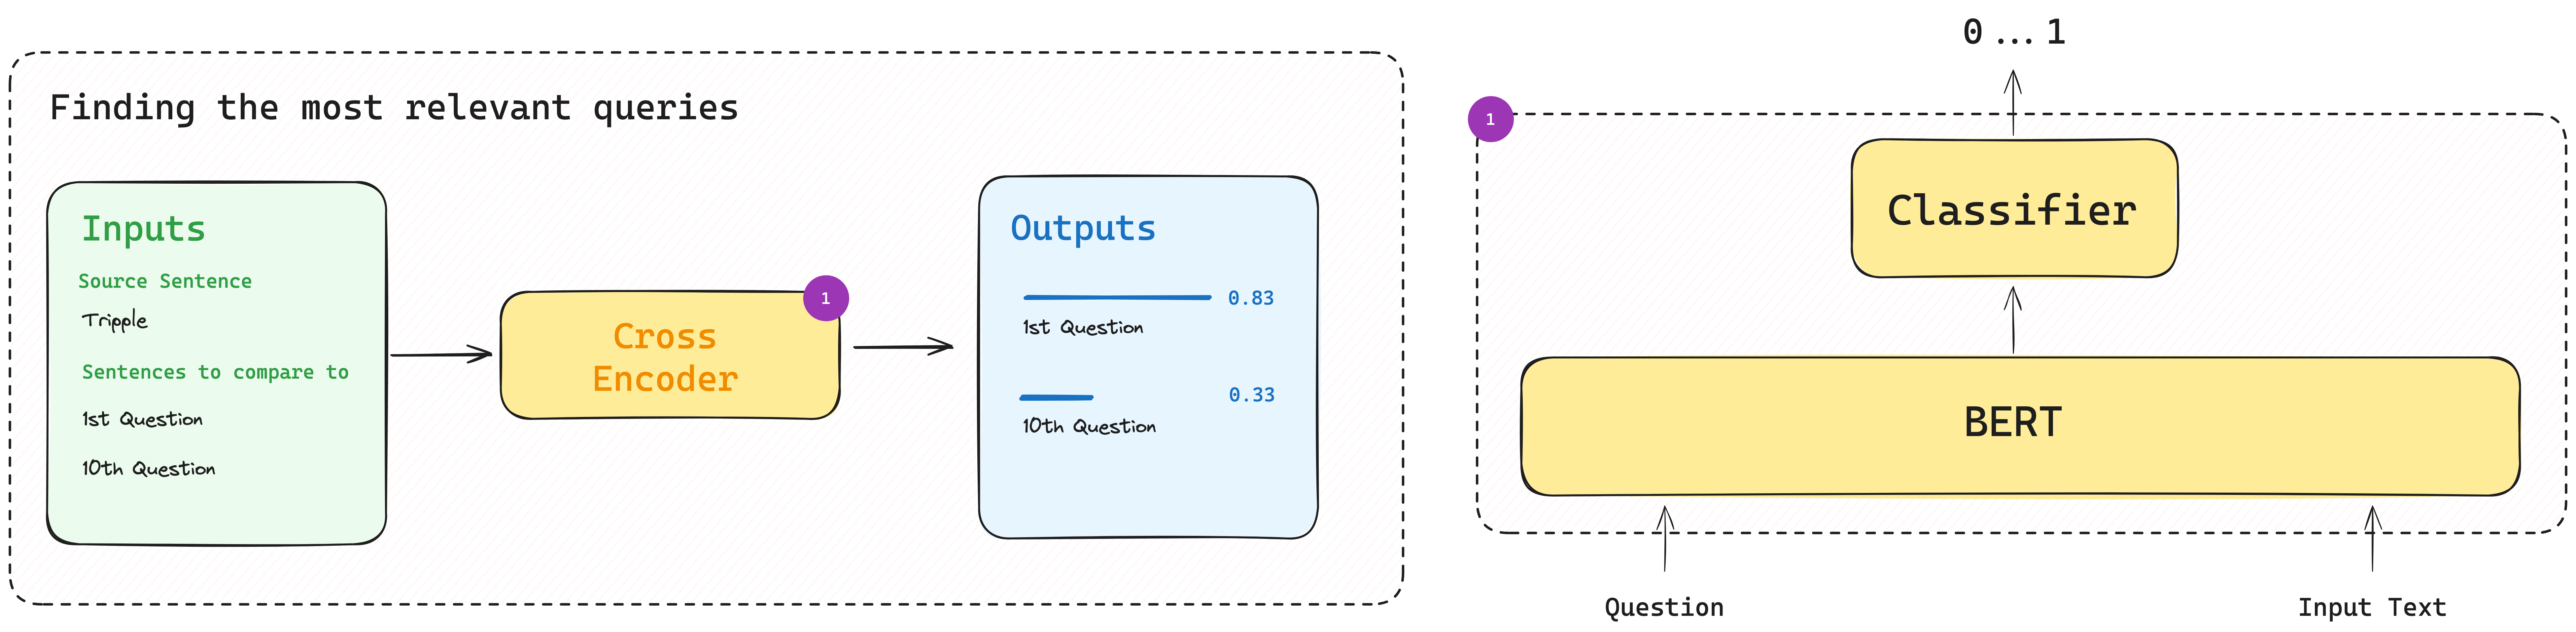
\includegraphics[width=\textwidth]{res/Cross-Encoder}
    \end{minipage}
    \caption{Cross-Encoder component, which assesses the relevance of generated questions by taking multiple input pairs and assigning a relevance score to each, supporting question evaluation and refinement.}
    \label{fig:cross-encoder-articture}
\end{figure}

Key features of the Cross-Encoder include:

\begin{itemize}
    \item \textbf{Input Processing:}
    \begin{itemize}
        \item Source Sentence: The original input text.
        \item Sentences to Compare: Likely the 10 generated questions.
    \end{itemize}
    \item \textbf{Scoring Mechanism:} The Cross-Encoder assigns numerical scores (\eg, 0.83 as shown in the figure~\ref{fig:cross-encoder-articture}) to each question, indicating its relevance to the source sentence.
    \item \textbf{Comparative Analysis:} By processing all inputs simultaneously, the Cross-Encoder can perform nuanced comparisons between the original input and each generated question, as well as among the questions themselves.
\end{itemize}

In this case we use the \textit{jinaai/jina-reranker-v1-turbo-en}\footnote{\url{https://huggingface.co/jinaai/jina-reranker-v1-turbo-en}} model from the Hugging Face Transformers library.
This model is designed for blazing-fast re-ranking while maintaining competitive performance.
It leverages the power of JinaBERT~\cite{günther2024jinaembeddings28192token} model as its foundation.
The model employs a process known as knowledge distillation to attain exceptional speed and efficiency, making it the optimal selection for our pipeline.

\begin{figure}[ht!]
    \centering
    \begin{minipage}[b]{\textwidth}
        \centering
        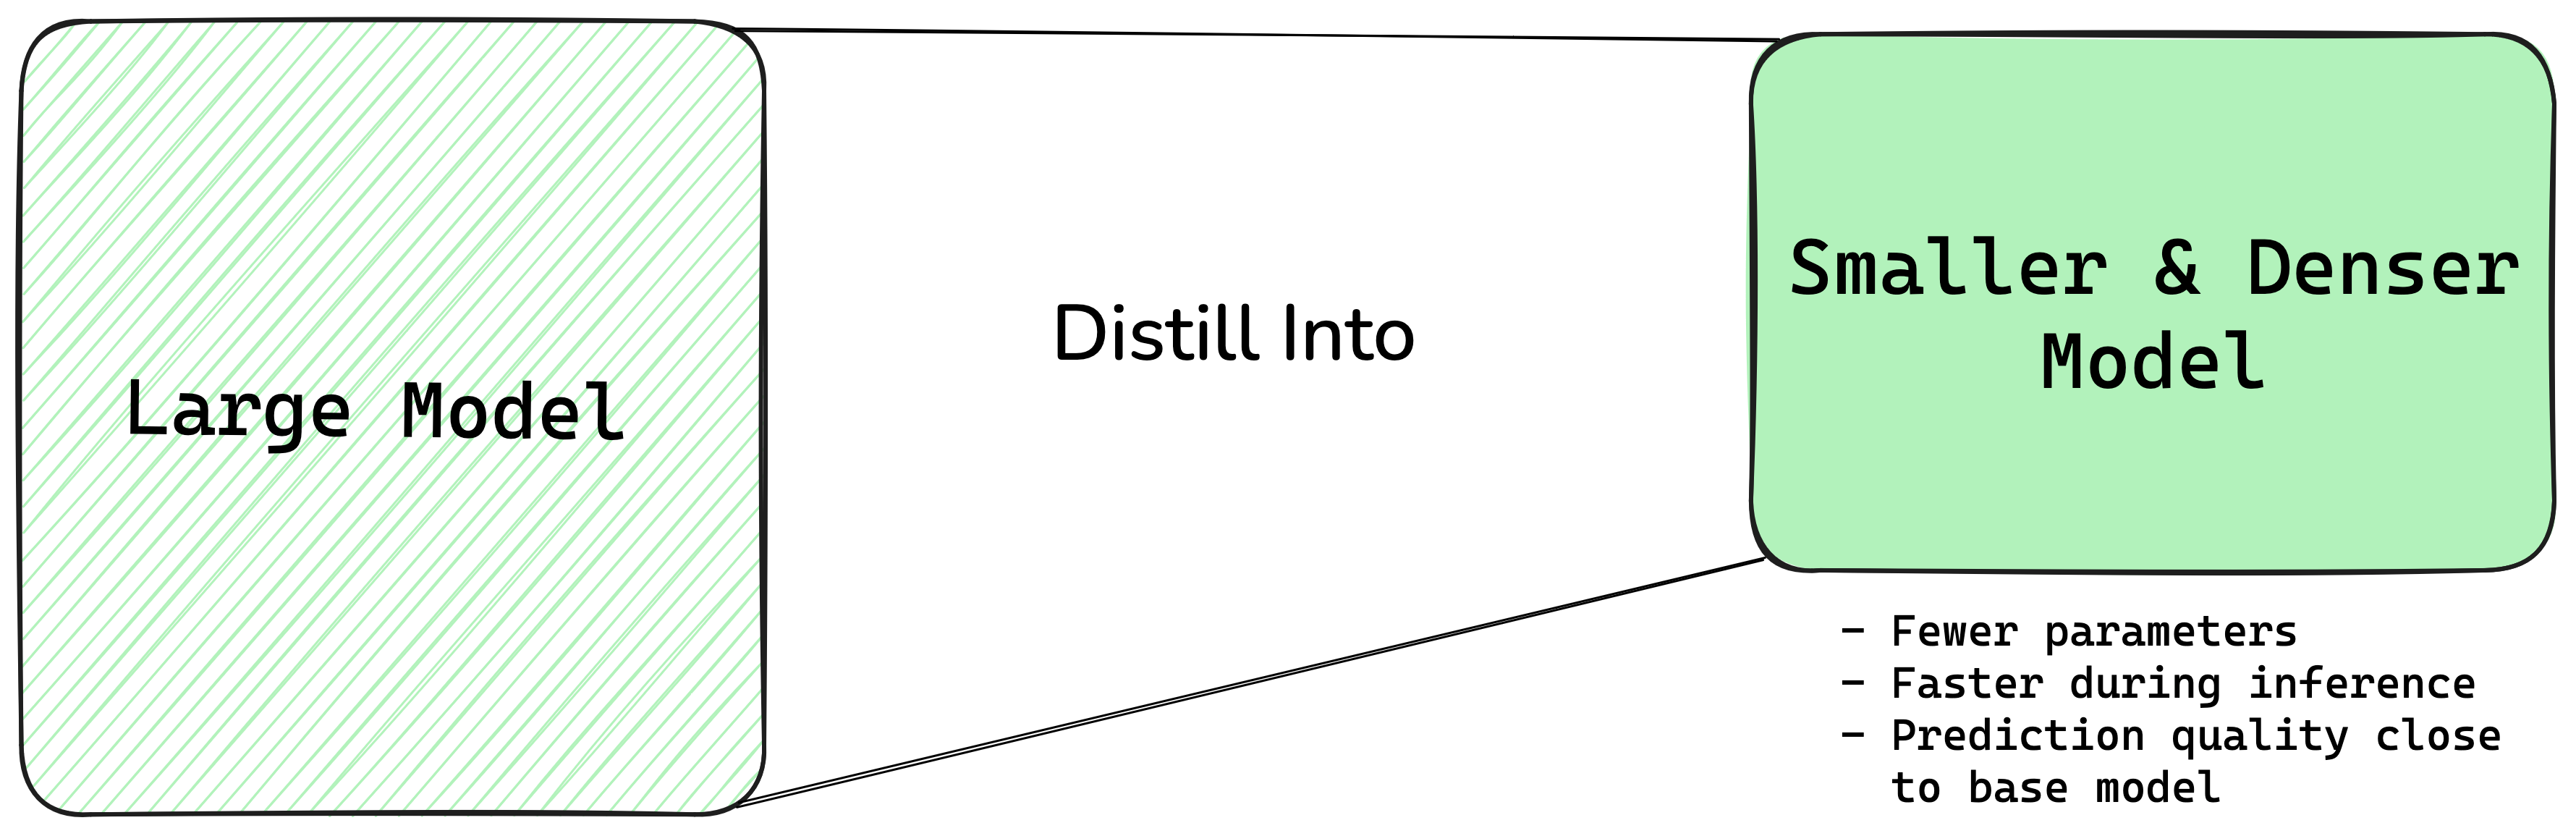
\includegraphics[width=0.7\textwidth]{res/knowledge-distill}
    \end{minipage}
    \caption{Knowledge Distillation Process for Enhanced Re-Ranking Efficiency}
    \label{fig:knowledge-distill}
\end{figure}
\subsection{Relevance Threshold and Sorting}\label{subsec:relevance-threshold-and-sorting}
Following the Cross-Encoder's scoring, the pipeline implements a crucial decision point:
\begin{itemize}
    \item \textbf{Sorting:} Questions are sorted based on their relevance scores, establishing a priority order for further processing.
    \item \textbf{Threshold Evaluation:} The system checks if the top question's score exceeds an upper threshold. This step ensures that only sufficiently relevant questions proceed further in the pipeline.
    \item \textbf{Feedback Loop:} If the threshold is not met, the process must loop back to generate new questions to adjust the existing ones, maintaining the quality of queries entering subsequent stages.
\end{itemize}

\begin{table}[h!]
    \noindent
    \caption{Example of generated questions by the Gemma2 model with relevance scores assigned by the Jina Re-ranker Cross-Encoder.}
    \resizebox{\textwidth}{!}{
        \begin{tabular}{llc}
            \toprule
            \textbf{Input} & \textbf{Question} & \textbf{score} \\
            \midrule
            \multirow{10}{*}{\shortstack[l]{\textit{Frédéric Passy} \\ \textit{award} \\ \textit{Nobel Peace Prize}}} & Who was awarded the Nobel Peace Prize? & 0.7458 \\
            & What award did Frédéric Passy receive? & 0.7121 \\
            & Is Frédéric Passy a Nobel laureate? & 0.8706 \\
            & In what category was the Nobel Peace Prize awarded to Frédéric Passy? & \textbf{0.9491} \\
            & Who is known for receiving the Nobel Peace Prize? & 0.5823 \\
            & What is the name of the award received by Frédéric Passy? & 0.6318 \\
            & Is Frédéric Passy a recipient of the Nobel Prize in any field? & 0.7652 \\
            & Who was recognized for his work towards peace? & 0.1457 \\
            & What is the significance of the award given to Frédéric Passy? & 0.6036 \\
            & Is there a Nobel laureate with the name Frédéric Passy? & 0.8505 \\
            \bottomrule
        \end{tabular}}
    \label{tab:Question scoring}
\end{table}

\section{Information Retrieval Mechanisms}\label{sec:information-retrieval-mechanisms}
The Information Retrieval Mechanisms are an essential element of our pipeline, connecting query processing and content synthesis.
This phase is tasked with gathering relevant data from internal and external sources, thereby establishing a comprehensive data repository for further analysis and response formulation.
The mechanisms employed in this phase are designed to ensure breadth, depth, and relevance in the retrieved information.

\subsection{Google Search Integration}\label{subsec:google-search-integration}
A key feature of our information retrieval process is the integration of Google Search capabilities, as prominently displayed in the pipeline diagram.
This integration serves to expand the information horizon beyond the confines of our internal Knowledge Graph Dataset.
Key aspects of this integration include:

\begin{itemize}
    \item \textbf{Query Submission:} The system submits the $N$ top questions (where $N$ is a predefined number) along with the main question to Google Search. This approach ensures a multi-faceted search that captures various aspects of the original query.
    \item \textbf{Result Fetching:} As indicated in the diagram, the system retrieves the top 100 search results. This number strikes a balance between comprehensiveness and computational efficiency.
    \item \textbf{Dynamic Information Access:} By leveraging Google Search, the system gains access to up-to-date information, complementing the more static nature of the internal Knowledge Graph.
    \item \textbf{Diverse Source Types:} Google Search results typically include a variety of source types (\eg, websites, news articles, academic papers), enriching the diversity of the retrieved information.
\end{itemize}

\begin{figure}[ht!]
    \centering
    \begin{minipage}[b]{\textwidth}
        \centering
        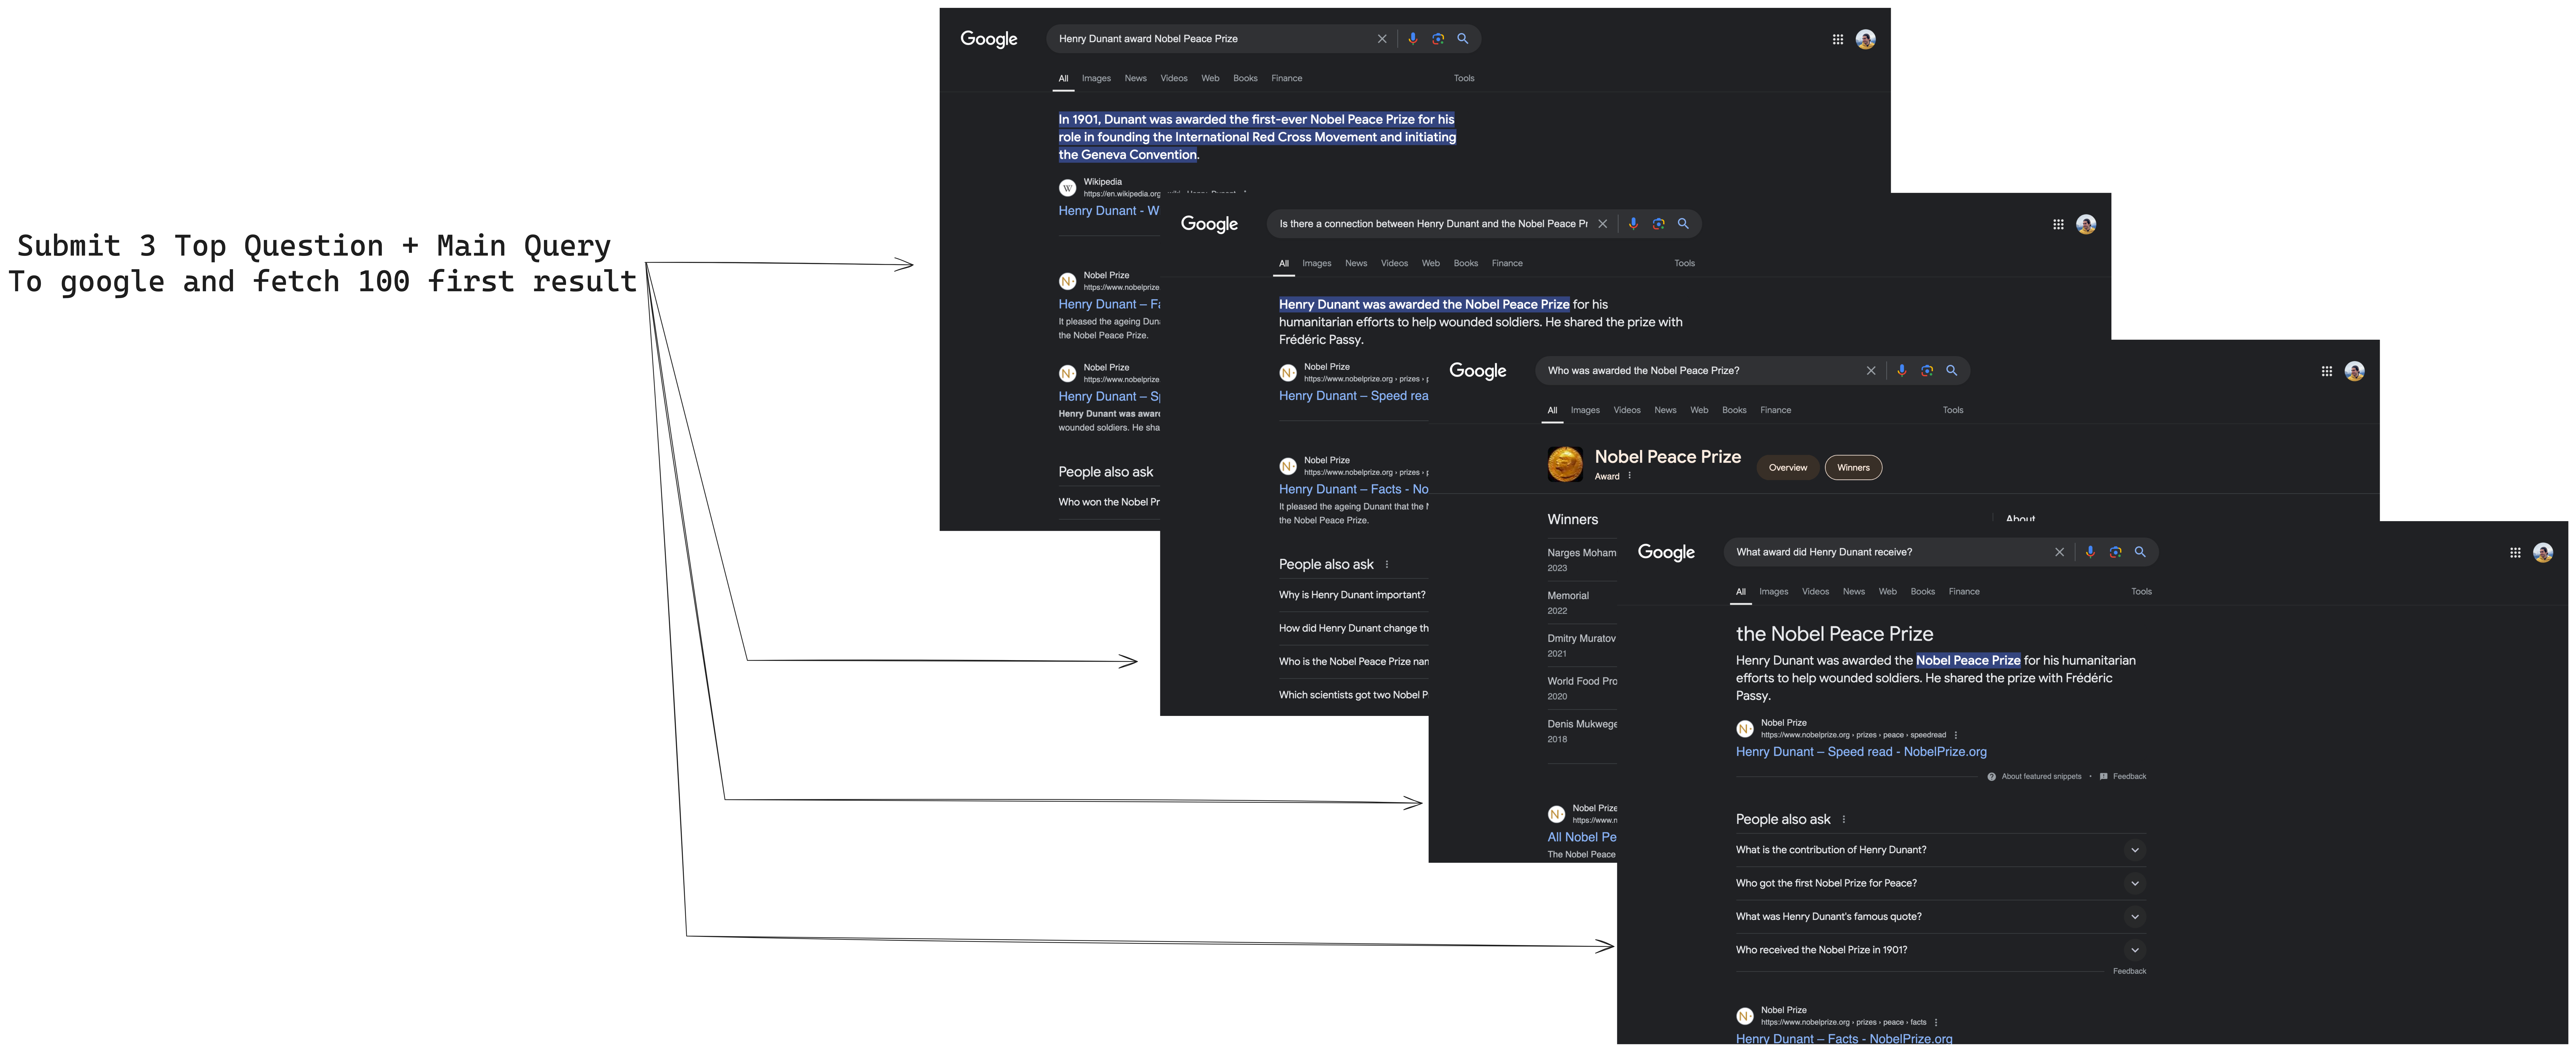
\includegraphics[width=\textwidth]{res/Google-Search-Result}
    \end{minipage}
    \caption{Fetching results from Google Search engine for top $N$ questions and the main knowledge graph query.}
    \label{fig:google-search-result}
\end{figure}

Implementation considerations:
\begin{itemize}
    \item The system may employ proxies or other mechanisms to manage rate limits and ensure uninterrupted access to search results.
    \item The search query may be customized based on the specific requirements of the pipeline, such as language restrictions, geolocation preferences, or result quantity. parameters are \textit{lr}, \textit{hl}, \textit{gl}, and \textit{num}.
\end{itemize}

Take note that the code base is generic, and it means that you can use any search engine, not only Google Search.

\subsection{Process and Extract Links}\label{subsec:process-and-extract-links}
Following the retrieval of search results, the pipeline incorporates a crucial step of processing and extracting links from the gathered information.
This process likely involves:
\begin{itemize}
    \item \textbf{Parsing \ac{HTML} Content:} Extracting relevant textual information from the retrieved web pages.
    \item \textbf{Link Analysis:} Identifying and cataloging hyperlinks within the content, potentially uncovering additional relevant sources.
\end{itemize}

After Parsing the HTML content of the Google Search results, the system use HTML selectors to extract the links from the search results.
In this case we also extract the title, url, description, price, date, duration, missing, rating, availability, and extra details from the search results.
Some of the information mentioned above may not be available as it depends on the search results.

Then there is a need to crawl the extracted links to get the content of the page, for doing this we use the Python library called \textit{GRequests}\footnote{\url{https://pypi.org/project/grequests/}}.
\textit{GRequests} is a Python library that combines the power of gevent for asynchronous I/O with the simplicity of the Requests library for HTTP operations. It allows developers to perform concurrent HTTP requests easily, significantly speeding up operations that involve multiple API calls or web scraping tasks.

\begin{lstlisting}[language=Python, caption=Crawling the extracted URLs, label=lst:crawling-urls]
import os
import grequests
from fake_useragent import UserAgent

ua = UserAgent(
    os=['windows'],
    browsers=["chrome", "edge", "firefox"],
    platforms=["pc"]
)

urls = [...List of Extracted URLs...]

rs = [
    grequests.get(u['url'],
    timeout=3, headers={"User-Agent": ua.random}) for u in urls
]
for index, response in grequests.imap_enumerated(rs, size=50):
    if response is None or response.status_code != 200:
        continue
    # Process the response content ...
\end{lstlisting}

There are several faults in the mentioned approach~\ref{lst:crawling-urls} that need to be addressed:
\begin{itemize}
    \item \textbf{Site generated with javascript:} The provided approach does not handle sites that are generated with JavaScript and require dynamic rendering.
    \item \textbf{Protection against scraping:} Sites may have protection mechanisms against scraping, such as CAPTCHAs or IP blocking or behind spam protection services.
    \item \textbf{Login required:} Some sites require login credentials to access the content.
\end{itemize}

We can use the \textit{Selenium}\footnote{\url{https://www.selenium.dev/}} library to handle the first issue, and for the second and third issues, we can use the \textit{Scrapy}\footnote{\url{https://scrapy.org/}} library, but we stick with the provided approach for simplicity and speed.

With the extracted content, the system can now proceed to the next stage of the pipeline, where the information is further processed and analyzed.
For extracting the content of the page, as our webpage are from vast sources, we need to use a robust and efficient library to extract the content of the page.
We use \textit{newspaper4k}\footnote{\url{https://newspaper4k.readthedocs.io/en/latest/}} library to extract the content of the page.
\textit{newspaper4k} is a Python library designed for extracting and parsing newspaper articles. It's an updated and improved version of the original newspaper3k library, offering enhanced functionality and compatibility with modern Python versions.

Key features of the \textit{newspaper4k} library include:
\begin{itemize}
    \item \textbf{Article Extraction:} Easily extract articles from news websites.
    \item \textbf{Multi-language Support:} Capable of processing articles in various languages.
    \item \textbf{Full-text Extraction:} Extracts the full text of articles, removing ads and extraneous content.
    \item \textbf{Keyword Extraction:} Automatically identifies key topics and keywords from articles.
    \item \textbf{Summary Generation:} Creates concise summaries of article content.
    \item \textbf{Metadata Parsing:} Extracts metadata such as authors, publication dates, and tags.
    \item \textbf{Image Extraction:} Identifies and extracts images associated with articles.
\end{itemize}

\begin{figure}[ht!]
    \centering
    \begin{minipage}[b]{\textwidth}
        \centering
        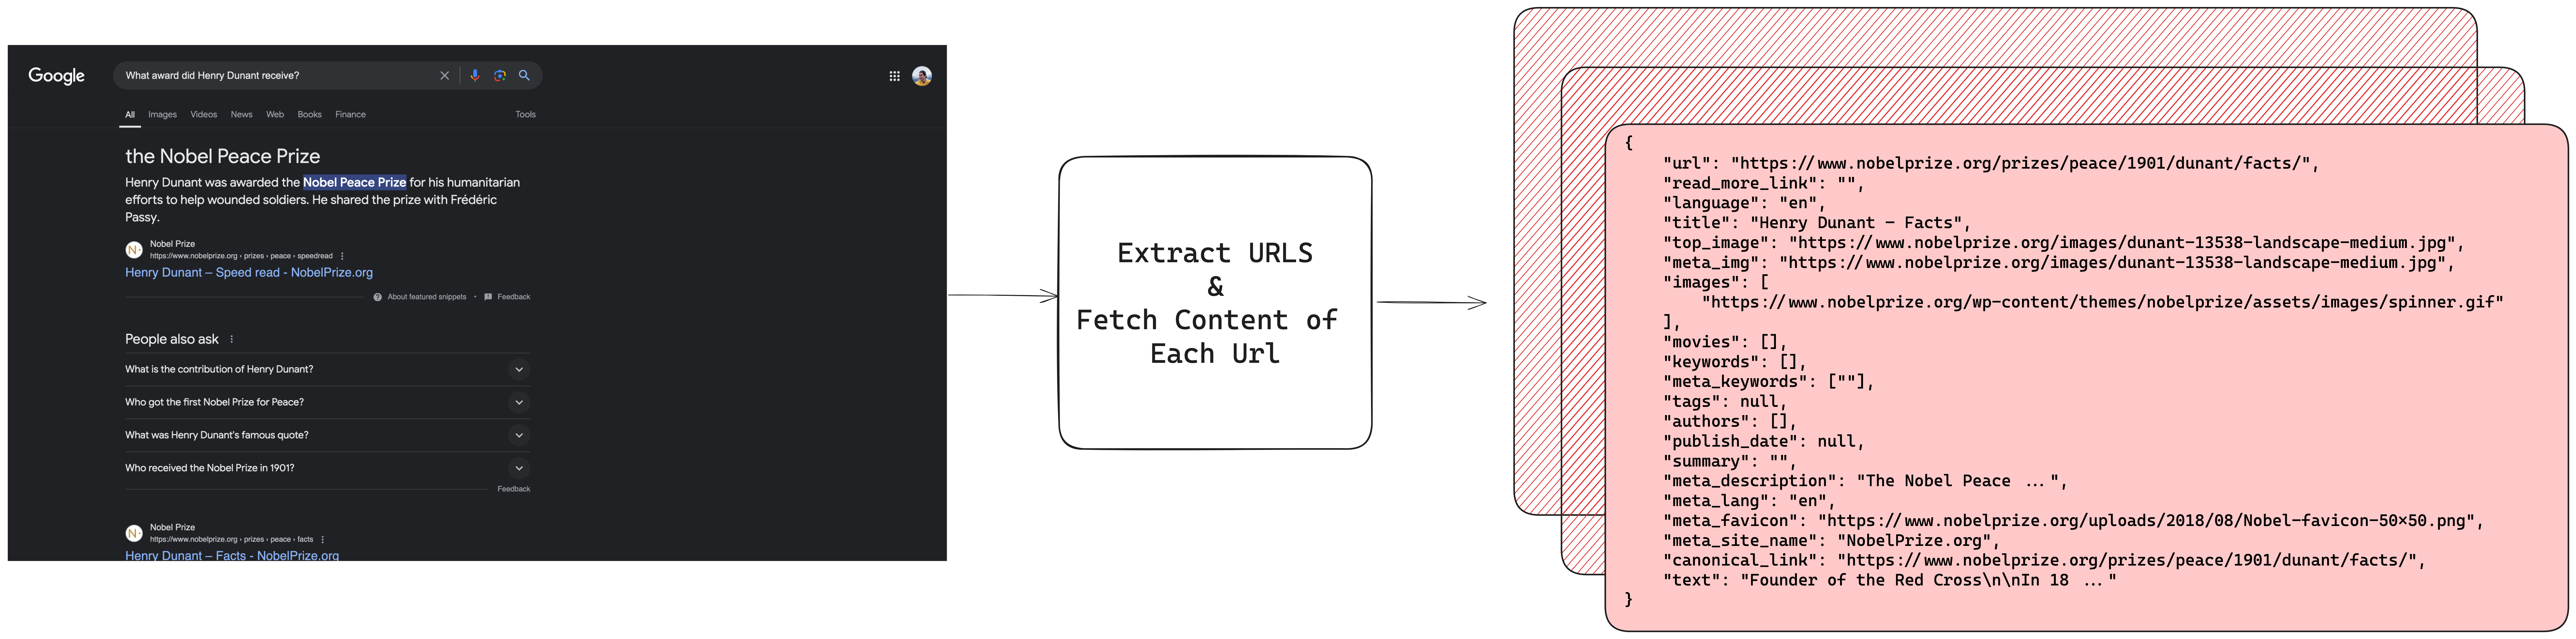
\includegraphics[width=\textwidth]{res/Google-Search-Result-Content}
    \end{minipage}
    \caption{Extracted content from the crawled URLs using newspaper4k library.}
    \label{fig:google-search-result-content}
\end{figure}

For our purpose, we only use the text content of the page.
\subsection{Data Pool Creation}\label{subsec:data-pool-creation}
The processed and extracted information culminates in the creation of a data pool, a centralized repository of relevant information that serves as the foundation for subsequent stages of the pipeline.

Key features of the data pool include:
\begin{itemize}
    \item \textbf{Structured Storage:} Organizing the retrieved information in a format that facilitates efficient querying and analysis.
    \item \textbf{Source Diversity:} Maintaining a balance between information from web searches and the internal Knowledge Graph.
    \item \textbf{Relevance Scoring:} Potentially implementing a scoring system to prioritize more relevant or authoritative pieces of information within the pool.
    \item \textbf{Deduplication:} Employing mechanisms to identify and merge duplicate or highly similar pieces of information to reduce redundancy.
\end{itemize}
\subsection{Data filtering}\label{subsec:data-filtering}
The data filtering process aims to refine our data pool by removing information from sources that are already part of creation of the Knowledge Graph.
This ensures the uniqueness and independence of our data, for example, when working with the FactBench dataset, we exclude data from the following sources: wikipedia.org, wikimedia.org, wikidata.org and other similar wiki-based platforms.

On the other hand, we just keep the top 10 relevant information for the pipeline using cross-encoders discussed in Section~\ref{subsec:cross-encoder-for-query-relevance-scoring}, this way we ensure about the quality of the data.
%More details about the data filtering process methodology are provided in the section~\ref{sec:document-selction}.

Specifically:
\begin{itemize}
    \item We start with a larger pool of data.
    \item We identify sources that are already the source of the Knowledge Graph.
    \item We remove any data points that come from these identified sources.
\end{itemize}

\section{Embedding and Retrieval Tasks}\label{sec:embedding-and-retrieval-tasks}
An important step in our pipeline is the Embedding and Retrieval Tasks, which connect machine-interpretable vector representations to unprocessed textual input.
This component is essential for improving the efficiency and accuracy of information retrieval and subsequent processing stages.

This section emphasizes embedding for retrieval tasks, specifically for small information segments, as depicted in the pipeline diagram.

\subsection{Embedding Techniques for Smaller Chunks}\label{subsec:embedding-techniques-for-smaller-chunks}
The pipeline employs advanced embedding techniques to transform textual data into dense vector representations, facilitating more efficient and semantically aware retrieval processes.

Key aspects of this embedding process include:
\begin{itemize}
    \item \textbf{Granularity:} The focus on "Smaller Chunks" suggests a fine-grained approach to embedding, where text is broken down into manageable units. This granularity allows for more precise retrieval and relevance assessment.
    \item \textbf{Dimensionality Reduction:} Transforming high-dimensional textual data into lower-dimensional vector spaces while preserving semantic relationships.
\end{itemize}

%we use the \textit{SentenceWindowNodeParser} to parse documents into single sentences per node.
%Each node also contains a \textit{"window"} with the sentences on either side of the node sentence.
%Then, after retrieval, before passing the retrieved sentences to the LLM, the single sentences are replaced with a window containing the surrounding sentences using the MetadataReplacementNodePostProcessor.
%This is most useful for large documents/indexes, as it helps to retrieve more fine-grained details.
%
%\begin{figure}[ht!]
%    \centering
%    \begin{minipage}[b]{\textwidth}
%        \centering
%        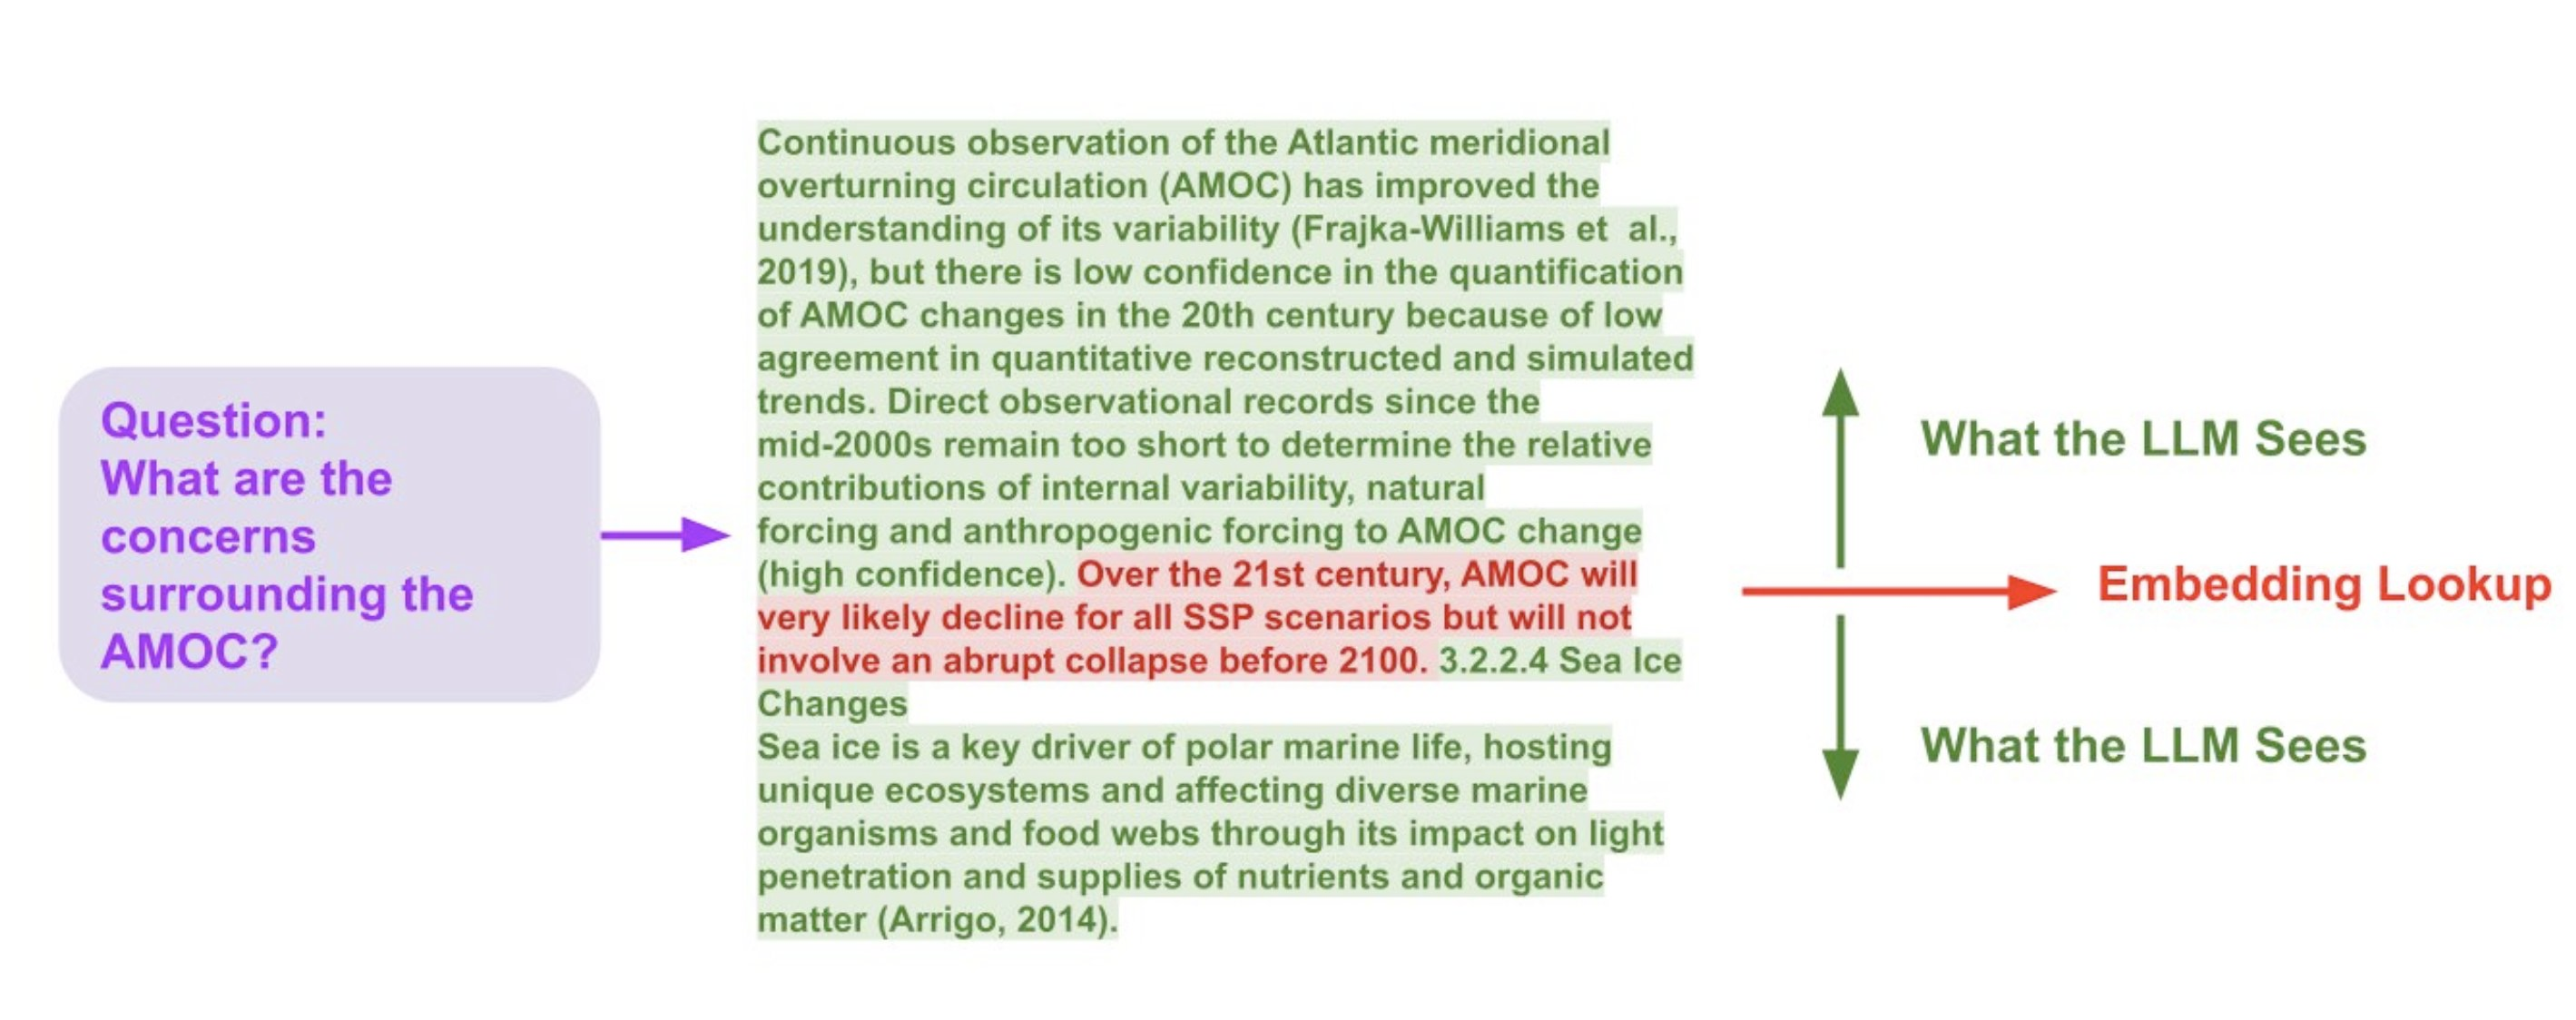
\includegraphics[width=\textwidth]{res/window-ret}
%        \caption{Node sentence window replacement~\cite{liu2023tweet}}
%        \label{fig:window-ret}
%    \end{minipage}
%\end{figure}
%
%There is example of the \textit{SentenceWindowNodeParser} and \textit{MetadataReplacementNodePostProcessor} in the Appendix~\ref{sec:chunking:sliding-window}.

\subsubsection{Challenges and Considerations}
Several challenges and considerations are inherent in the Embedding and Retrieval Tasks:
\begin{itemize}
    \item \textbf{Multilingual Support:} Extending embedding capabilities to support multiple languages, potentially through multilingual or language-agnostic models.
    \item \textbf{Embedding Interpretability:} Balancing the trade-off between the performance of dense embeddings and the interpretability often associated with sparse representations.
    \item \textbf{Temporal Dynamics:} Addressing the challenge of embedding temporally sensitive information and ensuring retrieval mechanisms account for time-based relevance.
    \item \textbf{Scalability:} Designing the embedding and retrieval systems to efficiently handle growing volumes of data without compromising on speed or accuracy.
    \item \textbf{Ethical Considerations:} Mitigating potential biases inherent in pre-trained embedding models and ensuring fair representation across diverse topics and perspectives.
\end{itemize}

\subsection{Similarity Cutoff Strategy}\label{subsec:similarity-cutoff-strategy}
One of the most important aspects that is highlighted in the pipeline diagram is the "Similarity Cutoff Strategy," which is significant since it is responsible for filtering and prioritizing the information that is included.

This strategy likely involves:
\begin{itemize}
    \item \textbf{Threshold Definition:} Establishing a similarity threshold below which embedded chunks are considered insufficiently relevant or related to the query or context.
    \item \textbf{Similarity Metrics:} Employing appropriate similarity measures (\eg, cosine similarity, Euclidean distance) to quantify the relatedness between embedded representations.
    \item \textbf{Re-run Mechanism:} Potentially re-do the response generation process if the similarity cutoff is not met for all the documents and the response is not generated.
\end{itemize}

The Similarity Cutoff Strategy serves several critical functions:
\begin{itemize}
    \item \textbf{Noise Reduction:} Filtering out irrelevant or tangentially related information to improve the signal-to-noise ratio in subsequent processing stages.
    \item \textbf{Computational Optimization:} Reducing the volume of data processed in later stages, thereby enhancing overall system efficiency.
    \item \textbf{Relevance Enhancement:} Ensuring that only the most pertinent information is retained for query resolution and response generation.
\end{itemize}

It can be switched off if the dataset is small or if the similarity cutoff is not needed.

\section{LLMs}\label{sec:large-language-models-llms-in-the-pipeline}
\ac{LLMs} play a pivotal role in our advanced NLP pipeline, serving as the cornerstone for sophisticated information synthesis and response generation.
As illustrated in the pipeline diagram, multiple LLMs are employed, contributing to a robust and nuanced approach to question answering and information processing.

\subsection{Integration of Multiple LLMs}\label{subsec:integration-of-multiple-llms}
The pipeline incorporates multiple LLMs working in concert, a design choice that offers several significant advantages:
\begin{itemize}
    \item \textbf{Diversity of Perspectives:} By utilizing multiple models, the system can capture a broader range of interpretations and approaches to information synthesis.
    \item \textbf{Specialization:} Different LLMs may be fine-tuned or specialized for particular types of queries or domains, allowing for more targeted and accurate responses in specific contexts.
    \item \textbf{Robustness:} The multi-model approach provides redundancy and helps mitigate individual model biases or weaknesses.
    \item \textbf{Scalability:} Parallel processing of information through multiple LLMs can potentially improve the system's throughput and response time.
\end{itemize}

Implementation considerations:
\begin{itemize}
    \item \textbf{Model Selection:} Choosing a diverse set of LLMs that complement each other in terms of strengths and specializations.
    \item \textbf{Load Balancing:} Implementing efficient mechanisms to distribute workload across the available models.
    \item \textbf{Version Management:} Maintaining and updating multiple LLMs to ensure they remain current and aligned with the latest advancements in NLP.
\end{itemize}

For running open-source LLMs, we use \textit{Ollama}\footnote{\url{https://ollama.com/}}, Ollama is an open-source project that simplifies the process of setting up, running, and using LLMs locally on your machine.
It provides a user-friendly area for managing and interacting with various LLMs, making it easier for developers and enthusiasts to experiment with AI without relying on cloud services.
Under the hood, \textit{Ollama} is just an API server written in go that serves GGUF models via llama.cpp~\footnote{\url{https://github.com/ggerganov/llama.cpp}} and a centralized hub of models/settings.
Performance Considerations and Limitations of \textit{Ollama}:
\begin{itemize}
    \item Performance Considerations
    \begin{itemize}
        \item Performance depends on your hardware, especially CPU and GPU capabilities.
        \item Larger models require more RAM and storage space.
        \item GPU acceleration can significantly improve inference speed.
    \end{itemize}
    \item Limitations
    \begin{itemize}
        \item Resource intensive for larger models.
        \item May not match the performance of cloud-based solutions for some use cases.
        \item Limited to models that are compatible with Ollama's framework.
    \end{itemize}
\end{itemize}

\subsection{Roles of LLMs in the Pipeline}\label{subsec:roles-of-llms-in-the-pipeline}
Based on the pipeline diagram, the LLMs serve several crucial functions:
\begin{itemize}
    \item \textbf{Information Synthesis:} Integrating and coherently combining information from various sources.
    \item \textbf{Context Processing:} Analyzing and interpreting the broader context of queries and retrieved information to generate more accurate and relevant responses.
    \item \textbf{Reasoning and Inference:} Drawing logical conclusions and making inferences based on the available information, potentially finding the correctness of the knowledge graph.
\end{itemize}

The prompt template used for RAG approach reported in Appendix~\ref{sec:prompt-templates:rag}, we use the selected chunks from the previous steps to feed the LLMs context and also provide few examples to the LLMs to generate the better response.

\section{Voting System and Conflict Resolution}\label{sec:model-diversity-and-conflict-resolution}
Our state-of-the-art pipeline for natural language processing relies heavily on the integration of many models and the deployment of procedures to resolve conflicts.
To ensure robust and trustworthy outcomes, this section covers the ways adopted to resolve disputes and harness model diversity.

\subsection{Majority Voting System}\label{subsec:majority-voting-system}
A significant aspect of the LLM integration, is the establishment of a majority voting mechanism for response creation.

This method provides numerous advantages:
\begin{itemize}
    \item \textbf{Consensus Building:} By aggregating outputs from multiple models, the system can identify areas of agreement, potentially leading to more reliable responses.
    \item \textbf{Error Mitigation:} Outlier responses or errors from individual models can be identified and potentially filtered out through the voting process.
    \item \textbf{Confidence Scoring:} The degree of consensus among models can serve as a proxy for the confidence level of the generated response.
    \item \textbf{Handling Ambiguity:} In cases where there's no clear majority, the system can potentially flag the response as uncertain or requiring further clarification.
\end{itemize}

Implementation challenges:
\begin{itemize}
    \item \textbf{Weighting Mechanism:} Determining whether all LLMs should have equal weight in the voting process or if some models should be prioritized based on their specific strengths or reliability.
    \item \textbf{Threshold Setting:} Establishing the criteria for what constitutes a "majority" and how to handle cases with no clear consensus.
    \item \textbf{Combining Diverse Outputs:} Developing methods to meaningfully aggregate potentially disparate outputs from different models into a coherent final response.
\end{itemize}
The pipeline incorporates several mechanisms for resolving conflicts that may arise from divergent model outputs.

\subsection{Conflict Resolution Strategies}\label{subsec:conflict-resolution-strategies}
As previously discussed~\ref{subsec:majority-voting-system}, the system employs a majority voting approach among LLMs to determine the most appropriate response.
This serves as a primary conflict resolution mechanism, leveraging the wisdom of the collective to mitigate individual model errors or biases.
\subsubsection{Final Judge Implementation:}
A crucial component in the conflict resolution process is the "final judge" module, as indicated in the pipeline diagram.
This element plays a pivotal role in resolving conflicts and ensuring coherence in the system's outputs.

Key aspects of the final judge implementation:
\begin{itemize}
    \item \textbf{Conflict Identification:} Detecting discrepancies or contradictions in outputs from different models.
    \item \textbf{Resolution Mechanisms:} Using predefined rules or algorithms to determine the final output based on the majority voting results.
    \item \textbf{Tie-Breaking:} Implementing strategies for scenarios where the majority voting system results in a tie or lacks a clear consensus.
    \item \textbf{Consistency Enforcement:} Ensuring that the final output maintains logical consistency and aligns with established knowledge bases.
\end{itemize}

The final judge module used a system named \textit{Adaptive Conflict Resolution}, which is an adaptive approach to conflict resolution based on the specified settings.

\subsubsection{Adaptive Conflict Resolution}
The pipeline demonstrates an adaptive approach to conflict resolution, as evidenced by the following feature:
"When two of the language models believe the answer is correct, and two believe it is wrong, we switch to a more advanced model, such as a commercial one or a model with more parameters."
There are two ways to apply this adaptive method: 1) Directly selecting commercial models (\eg, GPT-4), or 2) Using a more advanced, open-source model with more parameters (\eg, Gemma2:27b).
For the second option, we use the algorithm shown in Algorithm~\ref{alg:model-selection}.
This algorithm uses the mapping between the already used and final models to select the final model.
It utilizes parameters to identify either the most consistent model or the least consistent model to choose based on a majority vote across the entire system.

This adaptive strategy offers several advantages:
\begin{itemize}
    \item \textbf{Escalation Mechanism:} Provides a structured approach for handling ambiguous cases where simpler resolution methods are insufficient.
    \item \textbf{Resource Optimization:} Reserves the use of more advanced (and potentially more computationally expensive) models for cases that truly require their capabilities.
    \item \textbf{Accuracy Enhancement:} Leverages more sophisticated models to resolve complex conflicts, potentially leading to higher-quality outputs in challenging scenarios.
    \item \textbf{Flexibility:} Allows for the integration of specialized or proprietary models in a targeted manner, enhancing the system's overall capabilities without relying on these models for every query.
\end{itemize}

Implementation challenges:
\begin{itemize}
    \item \textbf{Threshold Definition:} Determining the exact criteria for when to invoke the more advanced models.
    \item \textbf{Model Selection:} Choosing which advanced model to use based on the nature of the conflict and the query context.
    \item \textbf{Integration:} Ensuring smooth handover and result incorporation from the advanced models back into the main pipeline.
\end{itemize}

\begin{algorithm}
    \footnotesize
    \caption{Resolve Ties in Majority Voting System}
    \begin{algorithmic}[1]
        \Require
        \Statex $modelScores$ - A list of consistency scores for each model
        \Statex $finalJudger$ - A dictionary mapping file indices to final model
        \Statex $atLeast$ - A boolean flag:
        \Statex \hspace{1em} True: select model with the highest agreement score
        \Statex \hspace{1em} False: select model with the lowest agreement score

        \Procedure{ProcessFiles}{$modelScores, finalJudger, atLeast$}
            \If{$atLeast$ is True}
                \State $maxScore \gets $ maximum score in $modelScores$
                \State $candidates \gets $ indices with score equal to $maxScore$
            \Else
                \State $minScore \gets $ minimum score in $modelScores$
                \State $candidates \gets $ indices with score equal to $minScore$
            \EndIf

            \State $chosenIndex \gets $ random choice from $candidates$
            \State \Return $finalJudger[chosenIndex]$
        \EndProcedure
    \end{algorithmic}\label{alg:model-selection}
\end{algorithm}
\section{Performance Report}\label{sec:performance-report}
In Tables~\ref{tab:pipeline-performance-report},~\ref{tab:pipeline-performance-report-2}, we provide a detailed performance report, highlighting key metrics that demonstrate the pipeline's efficiency.
Other sections of the pipeline, such as RAG and conflict resolution mechanisms, will be evaluated in future chapters.
\begin{table}[ht!]
    \noindent
    \caption{Performance of our LLM-based tasks in production, generated by Openlit with Gemma2 model.}
    \resizebox{\textwidth}{!}{
        \begin{threeparttable}
            \begin{tabular}{lcc}
                \toprule
                \textbf{Task} & \textbf{Avg. Request Time}\tnote{*} & \textbf{Avg. tokens per request} \\
                \midrule
                Human understandable text~\ref{subsec:human-understandable-text-generation} & 1.3164 sec & 343.16 \\
                Question Generation~\ref{subsec:question-formulation-techniques} & 9.6076 sec & 672.58 \\
                \bottomrule
            \end{tabular}
            \begin{tablenotes}
                \item[*] The average time is calculated on the Macbook Pro with M2 max chip and 32GB of RAM\@.
            \end{tablenotes}
        \end{threeparttable}}
    \label{tab:pipeline-performance-report}
\end{table}
\begin{table}[ht!]
%    \noindent
    \centering
    \caption{Performance of our information retrieval mechanisms.}
    \begin{threeparttable}
        \begin{tabular}{lc}
            \toprule
            \textbf{Task} & \textbf{Avg. Time}\tnote{*} \\
            \midrule
            Sorting the questions by similarity~\ref{subsec:cross-encoder-for-query-relevance-scoring} & 0.013 sec \\
            Get documents (Google pages)~\ref{subsec:google-search-integration} & 3.6 sec \\
            Fetch documents for each triple~\ref{subsec:process-and-extract-links} & 350 sec \\
            \bottomrule
        \end{tabular}
        \begin{tablenotes}
            \item[*] The average time is calculated on the unix based server with 2 cores and 4GB of RAM\@.
        \end{tablenotes}
    \end{threeparttable}
    \label{tab:pipeline-performance-report-2}
\end{table}

\section{Pipeline Flow and Decision Points}\label{sec:pipeline-flow-and-decision-points}
The architecture of our pipeline is characterized by a sophisticated flow of information and a series of critical decision points.
This structure enables the system to process complex queries, retrieve and synthesize relevant information, and generate accurate responses.
This section provides a comprehensive analysis of the pipeline's flow and the key decision points that guide the processing of information.

The pipeline flow can be broadly categorized into several main stages, each with its own set of processes and decision points:
\begin{itemize}
    \item Input Processing and Query Generation
    \item Information Retrieval and Enrichment
    \item Embedding and Relevance Assessment
    \item Multi-Model Processing and Synthesis
    \item Conflict Resolution and Final Output Generation
\end{itemize}
Let's examine each of these stages in detail in table~\ref{tab:pipeline-decision-points}, focusing on the flow of information and the critical decision points within each.
\begin{table}[ht!]
    \noindent
    \caption{Comprenhensive list of decision points in the pipeline flow.}
    \resizebox{\textwidth}{!}{
        \begin{tabular}{lp{11cm}}
            \toprule
            \textbf{Component} & \textbf{Decision Point} \\
            \midrule
            \multicolumn{2}{c}{\colorbox{pink}{\textit{Input Processing and Query Generation}}} \\
            Knowledge Graph Dataset Integration & Extent and nature of knowledge graph integration based on input complexity. \\
            Human-Understandable Text Generation & Selection of the most appropriate natural language generation technique based on input and context. \\
            Question Generation & Assessment of the quality and relevance of generated questions. \\
            Cross-Encoder for Query Relevance & Determination of whether the top question score exceeds the upper threshold. \\
            \hline
            \multicolumn{2}{c}{\colorbox{pink}{\textit{Information Retrieval and Enrichment}}}  \\
            Information Source Selection & Determining the most relevant and reliable sources for information retrieval. \\
            Google Search Integration & Balancing between the breadth of search (number of questions submitted) and depth (number of results retrieved). \\
            Process and Extract Links & Determining the relevance and quality of extracted information for inclusion in the data pool. \\
            Data Pool Creation & Structuring the data pool for optimal accessibility in subsequent stages. \\
            \hline
            \multicolumn{2}{c}{\colorbox{pink}{\textit{Embedding and Relevance Assessment}}} \\
            Embedding for Retrieval Tasks & Selection of the most appropriate embedding technique based on the nature of the data. \\
            Similarity Cutoff Strategy & Determination of the similarity cutoff threshold. \\
            Context Processing & Determining the optimal chunk size and processing method. \\
            \hline
            \multicolumn{2}{c}{\colorbox{pink}{\textit{Multi-Model Processing and Synthesis}}} \\
            Parallel LLM Processing & Allocation of specific tasks or aspects of the query to different models based on their strengths. \\
            Synthesis of Information & Determination of the method of synthesis (e.g., concatenation, abstraction, or hybrid approaches). \\
            Majority Voting System & Assessment of the level of agreement among models. \\
            \hline
            \multicolumn{2}{c}{\colorbox{pink}{\textit{Conflict Resolution and Final Output Generation}}} \\
            Conflict Identification & Determination of the threshold for what constitutes a significant conflict requiring resolution. \\
            Adaptive Model Selection & When two models believe the answer is correct and two believe it's wrong, switching to a more advanced model. \\
            Selection of Commercial Models & Choose the commercial model based on the user specified settings. \\
            Final Judge Implementation & Determination of the final response based on aggregated model outputs and conflict resolution results. \\
            Response Generation & Selection of the most appropriate format and level of detail for the response. \\
            \bottomrule
        \end{tabular}}
    \label{tab:pipeline-decision-points}
\end{table}

Several challenges and considerations are associated with managing the pipeline flow and decision points:
\begin{itemize}
    \item \textbf{Computational Efficiency:} Balancing the depth of processing at each stage with the need for timely responses.
    \item \textbf{Error Propagation:} Ensuring that errors or biases introduced at early stages don't disproportionately affect the final output.
    \item \textbf{Adaptability:} Designing decision points that can adapt to different query types and complexity levels.
    \item \textbf{Transparency:} Maintaining traceability of decisions made throughout the pipeline for accountability and debugging purposes.
    \item \textbf{Scalability:} Ensuring that the pipeline can handle increasing query volumes without significant degradation in performance or accuracy.
\end{itemize}

In conclusion, the Pipeline Flow and Decision Points represent a complex yet well-structured approach to natural language processing and question answering.
By implementing a series of carefully designed stages and critical decision points, the system aims to process information in a manner that maximizes accuracy, relevance, and reliability.
The adaptive nature of the pipeline, particularly in its approach to conflict resolution and model selection, demonstrates a commitment to handling a wide range of query complexities and scenarios.
However, the intricate nature of this flow also underscores the importance of ongoing optimization, monitoring, and refinement to ensure that the system continues to perform effectively and ethically in the face of evolving challenges and requirements in the field of AI and natural language processing.

\section{Ethical Considerations and Limitations}\label{sec:ethical-considerations-and-limitations}
The development and deployment of advanced pipelines, such as the one described in this thesis, necessitate a thorough examination of ethical considerations and an acknowledgment of system limitations.
This section explores the ethical implications of our fact-checking system and discusses its inherent constraints.

\subsection{Ethical Considerations}\label{subsec:ethical-considerations}
While the pipeline diagram does not explicitly highlight ethical components, several aspects of the system raise important ethical considerations:

\subsubsection{Misinformation and Harmful Content}\label{subsubsec:misinformation-and-harmful-content}
The system's ability to synthesize information from various sources poses risks related to misinformation:
\begin{itemize}
    \item \textbf{Propagation of False Information:} Potential for the system to inadvertently spread misinformation present in retrieved data.
    \item \textbf{Generation of Harmful Content:} Risk of producing responses that could be considered harmful, offensive, or inappropriate.
\end{itemize}

\subsubsection{Environmental Considerations}\label{subsubsec:environmental-considerations}
The computational resources required to run multiple LLMs and process large volumes of data raise environmental concerns:
\begin{itemize}
    \item \textbf{Energy Consumption:} High energy usage associated with running complex AI models and large-scale data processing.
    \item \textbf{Carbon Footprint:} Environmental impact of the infrastructure required to support the pipeline.
\end{itemize}

\subsection{Limitations}\label{subsec:limitations}
Understanding and acknowledging the limitations of the system is crucial for ethical deployment and user trust:

\begin{table}[h!]
    \noindent
    \caption{Limitations of the pipeline, categorized by scope of knowledge.}
    \resizebox{\textwidth}{!}{
        \begin{tabular}{lp{11cm}}
            \toprule
            \textbf{Limitation} & \textbf{Description} \\
            \midrule
            \multicolumn{2}{c}{\colorbox{pink}{\textit{Scope of Knowledge}}} \\
            Temporal Limitations & The system's knowledge base and models have a cutoff date, potentially leading to outdated information. \\
            Domain Specificity & Gaps in specialized or niche areas of knowledge may limit performance. \\
            \hline
            \multicolumn{2}{c}{\colorbox{pink}{\textit{Language and Cultural Limitations}}} \\
            Language Coverage & Biases towards languages well-represented in training data, challenges in handling less common languages. \\
            Cultural Context & Limitations in understanding and responding to culturally specific queries or contexts. \\
            \hline
            \multicolumn{2}{c}{\colorbox{pink}{\textit{Reasoning and Inference Capabilities}}} \\
            Complex Reasoning & Challenges in handling queries requiring advanced logical reasoning or domain-specific expertise. \\
            Causal Understanding & Difficulties in inferring causal relationships. \\
            \hline
            \multicolumn{2}{c}{\colorbox{pink}{\textit{Handling of Ambiguity and Context}}} \\
            Contextual Nuances & Difficulties in capturing subtle contextual cues that humans naturally understand. \\
            Disambiguation & Challenges in resolving ambiguities in queries without additional user input. \\
            \hline
            \multicolumn{2}{c}{\colorbox{pink}{\textit{Real-time Adaptation}}} \\
            Static Knowledge Base & Limitations in adapting to real-time changes without system updates. \\
            Learning from Interactions & Inability to learn and improve from individual user interactions due to privacy and architectural constraints. \\
            \bottomrule
            \end{tabular}
    }
    \label{tab:pipeline-limitations}
\end{table}